\section{Designing Energy Efficient Neural Networks}\label{algoback}

While DNNs deliver the state of the art accuracy on many AI tasks, it comes at the cost of high computational complexity.
Therefore, the progress in Deep learning is limited by how fast the NNs can be computed.
For real time applications, it requires low latency inference where small number of images can be classified quickly.
However, we cannot rely on processing manufacturing companies to provide better CPUs as Moore's law is no longer providing extra computation.
Accordingly, techniques that enable efficient processing of DNNs to improve energy efficiency and throughput without sacrificing the application accuracy or increasing hardware cost are critical to the wide deployment of DnNs in AI systems.




Training and Inference Efficiency:
The storage requirements are higher to store the intermediary values and output of backprop; Precision required for rtaining training is higher than precision required for inference.
While there are some techniques to improve the efficiency of training, we focus only on improving the efficiency of prediction stage.Computation requirement for training and inference vary where training requires powerful resources taking days and multiple hours in the cloud.
While inference can be performed locally on the edge(IoT or mobile).
In many applications, it is desirable to have computation near the sensors (edge computing) to reduce the commnication latency and cost and lowering the security risks of processing senstitive data on the cloud.
However, many of the embedded devices on the edge have stringent energy conumption, computation and memory limitations requiring efficient processing of NNs.
The key metrics for embedded machine learning include accuracy (utility), energy consumption, throughput and cost.

Energy consumption is often dominated by data movemet as memory access consumes singificantly more energy than computation[M Horowitz: COmputing's energy problem and what we can do about it]
The cost is dictated by the memory consumption or storage required on the chip.
Throughput which is dictated by the amount of computation and increases with the dimensionality of the data.

While specialised hardware addresses these issues fby optimising the data flow, minimising access to expensive levels of memeory and reuse at lower levels of memroy hierarcy[cite eyeriss paper], we only consider the joint algorith-hardware co-design techniques which aim to optimise the NNs for embedded devices.

In this work, we investigate the problem of performing privacy-preserving inference on neural networks. Let $\theta$ be the model parameters stored on the server, $x$ be the client's input, $y$ be the expected output and $f$ is the inference function to be computed. Given this, we want to compute the below function:

\begin{equation}
f(x,\theta)\rightarrow y
\end{equation}


\paragraph{Parameter.}
As our first observation, we present that the number of gates can be calculated as a function of the parameter size in the network. Thus, smaller parameter values result in lower of number gates to represent them. Table~\ref{tbl:gc_complexity} shows the number of total gates, non-XOR gates and communication required to design circuits for basic operations such as addition, multiplicaiton, greater than and so on. We observe that inputs with lesser bit sizes require smaller number of non-XOR gates, thereby exhibiting efficienct execution performance. Moreover, the number of bytes communicated are directly proportional to the
input size as well.

Neural networks have shown to exhibit high accuracies even with 8-bit or 16-bit precision and do not need to have 32 or 64-bit precision. Ideally, the lowest possible value that a parameter can take is 1 bit. Binary neural networks have achieved accuracies almost similar to those of standard networks for dataset such as MNIST, CIFAR and others.  This naturally aligns with our selected cryptographic primitive as each wire in garbled circuits represents 1 bit value.  Binarizing the model parameters further allows us to heavily use the free XOR, XNOR and NOT gates in garbled circuits. We present detailed information regarding the construction in Section~\cite{}.
Based on this observation, we propose the first optimization of reducing the parameter sizes. We reduce the parameter sizes in the network to design smaller garbled circuits while retaining the accuracy of the original model.

In this paper, we aim to answer the following research question:

{\em Whether it is possible to redesign neural network algorithms for secure computation while achieving acceptable accuracy and efficiency simultaneously?}

\paragraph{Structures.}
Next, we observe that the structure of the neural network itself heavily influences the number of gates in the circuit. Designing optimized circuits depends on several factors in the network architecture such as the number of layers in the network, number of neurons per layer, the connections between them and so on. For example, varying the number of kernels, stride size, padding  for convolutional layers directly affects the computation and communication cost of garbled circuits.
Further, we observe that deeper networks having small number of inputs at each layer are better suited for GC. We utilize these observations to modify the structure of neural networks while retaining inference accuracy comparable to standard models.

In designing our solution, we aim for the following main goals:

\begin{itemize}
\item {\em Privacy-}
The solution should preserve privacy of the model parameters $\theta$ from the users and that of $x$ and $y$ from the server.

\item {\em Accuracy-}
The drop in accuracy of the privately computed inference function should be minimum as compared to the accuracy of the model on plaintext data.

\item {\em Performance-}
The private computation should demonstrate acceptable performance overhead, preferably within a few milliseconds per inference request.

\end{itemize}


add section for energy efficiency for each of the efficient training algorithms.

Instead of using multiplication and addition circuits, we perform XNOR operations on the inputs followed by a bitcount operation. This reduces the overall number of non-XOR gates used to compute the operation. The equation can be represented as follows.

\begin{align}
\mathbf{x} \cdot \mathbf{w} =
N - 2\times\operatorname{bitcount}(\operatorname{xnor}(\mathbf{x}, \mathbf{w}))
\end{align}

As our main contribution, we show that neural network algorithms can be heavily optimized to execute efficiently using garbled circuits. We observe that the efficiency of evaluating an inference circuit depends on two key factors: the model parameters and the network structure.  With this observation,  selects optimal parameter size and network structure to guarantee acceptable {\em performance}. Last but not the least, to ensure high {\em accuracy} of the model,  uses an architecture search approach to find the best model with high accuracy and efficiency on garbled circuits.

In this paper, we provide directions to design neural networks for secure inference and low private computation overhead. We show that our optimized neural network architectures execute faster than Gazelle, the most efficient existing solution on privacy-preserving deep learning inference.


\pgfmathdeclarefunction{gauss}{2}{%
  \pgfmathparse{1/(#2*sqrt(2*pi))*exp(-((x-#1)^2)/(2*#2^2))}%
}


\begin{figure*}[ht!]
\begin{center}% note that \centering uses less vspace...
\resizebox{2\columnwidth}{!}{%
\begin{tabular}{lllll}


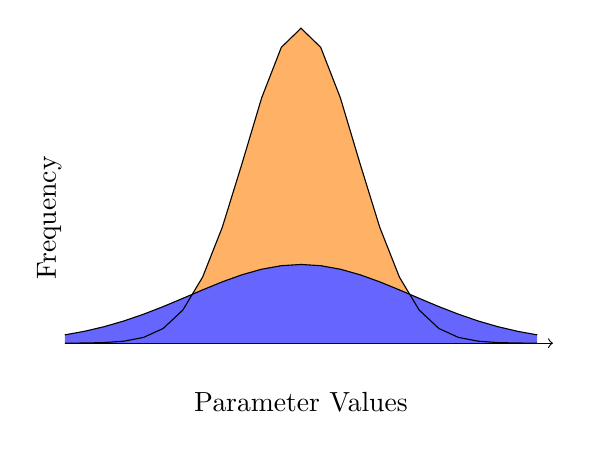
\begin{tikzpicture}
% define normal distribution function 'normaltwo'
\def\normaltwo{\x,{4*1/exp(((\x-3)^2))}}
\def\normal{\x,{1/exp(((\x-3)^2)/(4))}}


% Shade orange area underneath curve.
\fill [fill=orange!60] (0,0) -- plot[domain=0:6] (\normaltwo) -- (6,0) -- cycle;
\fill [fill=blue!60] (0,0) -- plot[domain=0:6] (\normal) -- (6,0) -- cycle;

% Draw and label normal distribution function
\draw[color=black,domain=0:6] plot (\normaltwo) node[right] {};
\draw[color=black,domain=0:6] plot (\normal) node[right] {};


% Optional: Add axis labels
\draw (-.2,2.5) node[left, rotate=90] {Frequency};
\draw (3,-.5) node[below] {Parameter Values};

% Optional: Add axes
\draw[->] (0,0) -- (6.2,0) node[right] {};
%\draw[->] (0,0) -- (0,5) node[above] {};

\end{tikzpicture} &


%
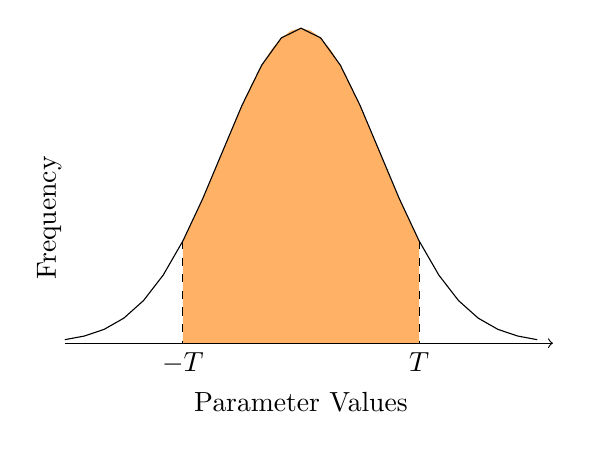
\begin{tikzpicture}
% define normal distribution function 'normaltwo'
\def\normaltwo{\x,{4*1/exp(((\x-3)^2)/2)}}

% input y parameter
\def\y{4.5}
\def\z{1.5}

% this line calculates f(y)
\def\fy{4*1/exp(((\y-3)^2)/2)}
\def\fz{4*1/exp(((\z-3)^2)/2)}

% Shade orange area underneath curve.
\fill [fill=orange!60] ({\z},0) -- plot[domain=1.5:4.5] (\normaltwo) -- ({\y},0) -- cycle;

% Draw and label normal distribution function
\draw[color=black,domain=0:6] plot (\normaltwo) node[right] {};

% Add dashed line dropping down from normal.
\draw[dashed] ({\y},{\fy}) -- ({\y},0) node[below] {$T$};
\draw[dashed] ({\z},{\fz}) -- ({\z},0) node[below] {$-T$};


% Optional: Add axis labels
\draw (-.2,2.5) node[left, rotate=90] {Frequency};
\draw (3,-.5) node[below] {Parameter Values};

% Optional: Add axes
\draw[->] (0,0) -- (6.2,0) node[right] {};
%\draw[->] (0,0) -- (0,5) node[above] {};

\end{tikzpicture} &





%
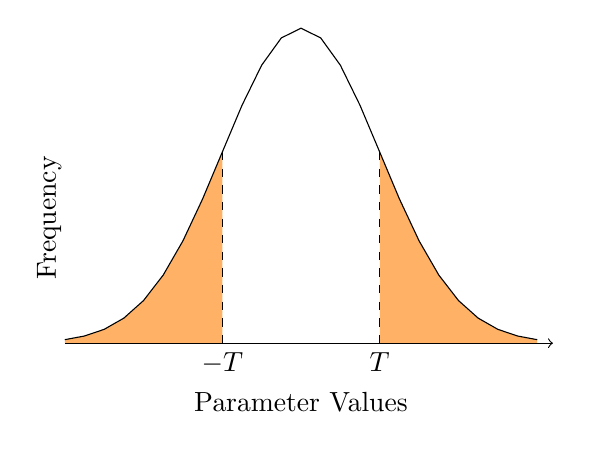
\begin{tikzpicture}
% define normal distribution function 'normaltwo'
\def\normaltwo{\x,{4*1/exp(((\x-3)^2)/2)}}

% input y parameter
\def\y{4}
\def\z{2}

% this line calculates f(y)
\def\fy{4*1/exp(((\y-3)^2)/2)}
\def\fz{4*1/exp(((\z-3)^2)/2)}

% Shade orange area underneath curve.
\fill [fill=orange!60] (0,0) -- plot[domain=0:2] (\normaltwo) -- ({\z},0)  -- cycle;
\fill [fill=orange!60] (4,0) -- plot[domain=4:6] (\normaltwo) -- (6,0)  -- cycle;

% Draw and label normal distribution function
\draw[color=black,domain=0:6] plot (\normaltwo) node[right] {};

% Add dashed line dropping down from normal.
\draw[dashed] ({\y},{\fy}) -- ({\y},0) node[below] {$T$};
\draw[dashed] ({\z},{\fz}) -- ({\z},0) node[below] {$-T$};


% Optional: Add axis labels
\draw (-.2,2.5) node[left,rotate=90] {Frequency};
\draw (3,-.5) node[below] {Parameter Values};

% Optional: Add axes
\draw[->] (0,0) -- (6.2,0) node[right] {};
%\draw[->] (0,0) -- (0,5) node[above] {};

\end{tikzpicture}

\end{tabular}
}
\caption{.}
\label{fig:loss}
\end{center}
\end{figure*}


\textbf{Machine and Deep Learning.}

\textit{Quantized Neural Networks}

One approach of improving efficiency for Neural Networks is through quantizing the parameter values and hence, reducing the precision of parameters number of bits required to represent the values in hardware \cite{Hubara:2017:QNN:3122009.3242044}.

A specific case of quantized Neural networks is using binary parameter and activation values\{-1,+1\} \cite{NIPS2016_6573}\cite{NIPS2015_5647}
For such binarized Neural Networks, the computation overhead due to matrix multiplication can be replaced by cheaper XNOR computation \cite{rastegari2016xnornet}\cite{DBLP:journals/corr/ZhouNZWWZ16}.
BNNs result in lower accuracy compared to full precision counterparts and several research papers and explored improving the accuracy-efficiency trade-off \cite{AAAI1714619}.
Ternary weighted Networks provide better accuracy compared to BNNs at the cost of higher precision with weights \{-W,0,+W\} where the threshold $W$ can be learned for higher performance \cite{DBLP:journals/corr/ZhuHMD16}\cite{Li2016TernaryWN}

\begin{algorithm}
\begin{algorithmic}
    \FOR{$k=1$ to $L$}
        \STATE $W_k^b \leftarrow {\rm Binarize}(W_k)$
        \STATE $a_k \leftarrow a_{k-1}^b W_k^b$
        \IF{$k < L$}
            \STATE $a_k^b \leftarrow {\rm Binarize}(a_k)$
        \ENDIF
    \ENDFOR

\end{algorithmic}
\caption{
Inference Stage of Binary Neural Network; Binarize() function is deterministic thresholding scheme; $W_k^b$ are the binarized weights($W_k$) and $a_k$ is the activation of the $k^{th}$ layer
}
\label{alg:train}
\end{algorithm}


\textit{Pruning.} \cite{Han:2015:LBW:2969239.2969366}


\textit{Efficient Architecture Design.} The design space for Neural Networks enables to find multiple models with different complexity but same accuracy.
Smaller Neural Networks allow to deploy on FPGA's and other low-powered devices with limited memory.
Two such Neural Network models are SqueezeNet \cite{DBLP:journals/corr/IandolaMAHDK16} and MobileNetV2 \cite{conf/cvpr/SandlerHZZC18} which are specifically designed to have less number of parameters and memory footprint.


\textit{Efficient Training Pipelines}

Dense sparse dense training \cite{DBLP:journals/corr/HanPNMTECTD16}
Model compression pipeline cobining pruning, quantization and huffman coding \cite{DBLP:journals/corr/HanMD15}
Huffman Coding is used for representation while storing in the hardware and in our experiments, we use pruning followed by quantization to achieve model compression.


Compact Network Architectures: The number of parameters and complexity of etwork can be optimized by careful design of the network architecture itself.
Here, instead of replacing larger filters with a set of smaller filters which have fewer weights in total when the filters are applied sequentially they have same overall receptive field.
For instance, one 5x5 filter can be replace with 2 3x3 filters. 1x1 convolutional layers can be used to reduce the number of channels in output feature map and hence the overall computation.
Forexample,32 ltersof1x1x64can transform an input with 64 channels to an output of 32 channels and reduce the number of  lter channels in the next layer to 32. SqueezeNet uses many 1 x 1  lters to aggressively reduce the number of weights [157]. It proposes a  re module that  rst “squeezes” the net- work with 1 x 1 convolution  lters and then expands it with multiple 1 x 1 and 3 x 3 convolution  lters.
It achieves an overall 50x reduction in the number of weights compared to AlexNet, while maintaining the same accuracy
Replace 3x3 filters with 1x1 filters.Given a budget of a certain number of convolutionfilters,  we will choose to ma
ecrease the number of input channels to 3x3 filters.Consider a convolution layerthat is comprised entirely of 3x3 filters. , to maintain a small total number of parametersin a CNN, it is important not only to decrease the number of 3x3 filters (see Strategy 1 above), butalso to decrease the number ofinput channelsto the 3x3 filters.  We decrease the number of inputchannels to 3x3 filters usingsqueeze layers, which we describe in the next section.
Downsample late in the network so that convolution layers have large activationmaps.In a convolutional network, each convolution layer produces an output activation map witha spatial resolution that is at least 1x1 and often much larger than 1x1.



Network Pruning: Neural Networks are generally overparameterised. Hence, a large amount of weights are redundant adn can be removed (set to zero) referred to as pruning.
Aggressive pruning, however, requires to finetune the model to ensure no loss in the accuracy. Typically, this is done by removing the least significant nodes in the network by computing a threshold using the senstitivity hyperparameter which is used to estimate the percentile of values.

\[
    f(W)=
\begin{cases}
    0, & \text{if } w\geq T\\
    0, & \text{if } w\leq -T\\
    w,  & \text{otherwise}
\end{cases}
\]

The original pruning requires the model to be retrained after pruning to restore accruacy while ensuring lower network size.
Further, computation on these sparse parameter matrices using specialized accelerators enable to avoid computation on 0's lower the computation complexity significantly and increasing the overall inference speed.
Prior work has indicated that over 80\% of the parameters can be pruned and the accuracy can be restored after retraining.

Sparsity: Sparsity reduces some of the values in the network close to zero replaces them as zero. This results in the distribution with two modes instead of a single gaussian distribution for the parameters.
The sparsity constraint ensures that the parameters in the middle are zeroed out while the parameter values near the tail end are updated.

\[
    f(W)=
\begin{cases}
    w, & \text{if } w\geq T\\
    w, & \text{if } w\leq -T\\
    0,  & \text{otherwise}
\end{cases}
\]

Sparse weights can be stored in a compressed format in the hardware using the compressed sparse row or column format which reduces the overall memory bandwidth[].
The decision on whether the computation is done is based on the parameter value which requires additional logic, i.e, replace output as zero without computation if parameter value is zero else perform the computation.
This also benefits in usage with SIMD or data parallel architectures and improves compression and reduces overall storage cost by using indices of weights with a zero values instead of actually storing zero values in the memory for each occurance.

Quantization reduces the precision of the operands while techniques such as pruning, sparsity reduce the number of model operation and model size.
Quantization maps parameters/activtions to a smaller set of quantization levels [qunaitized neural networks].
The ultimate goal is to minimize the error between the reconstructed data from hte quantized levels and the original data.
The number of quantized levels reflects the precision and ultimately the nuber of bits required to represent the data (log2(number of levels))
Reducing precision results in lower number of bits to represent the data which results in a lower storage cost (parameters) and/or computation cost (activation). less are and less energy [M Horowitz]
For instance, using kbits instead of 32 bits or 64 bits weights reduces the storage cost by 32/k or 64/k and hence, requires lower number of parameters to be read form the memory which further improves the energy efficiency by 32/kx or 64/kx.

The precision can be reduced aggresively to a single bit to get binary nets. Here, the weights  and activation are binarized during inference to take values \{-1,+1\} [binaryconnect, binarynet]. This allows to reduce the MAC operation to an XNOR however, with a singificant accuracy loss[xnor-net].
Several optimisaition have been considered to reduce the loss such as multiplying the outputs with a scaling factor to recover the dynamic range( weights become -w and w), keeping the first and last layer as 32 bit floating point precision and performing normatlisation before convolution to reduce the dynamic range of activations.
Further, hybrid and varying bit precision of weights and activations have been used in Dorefanet, HWGQnet and QNNs to reduce the qunatization loss.
Further, there are benefits for allowing weights to be zero (-w, 0, w) although this requires an additional bit per weight compared to binary weights, the sparsity can be used to reduce computation and storage cost [Ternary weight networks, trained ternary quantization].
Here, we consider two cases: uniform quanrization
Weight sharing forces several weight values to share a single value which reduces the number of unique weights in the model.
The weights are grouped using hashing function or k means algorithm and one value is assigned to each group.
A codebook is then built to map each grou of weights to its shared value. accordingly, the index to the corresponging group in the codebook is strored for each position n the filter rather than a eright value. This leads to a two step process to fetch the weights:
(a) read the group index from the weight memory and (b) using the griup index read the value of weight from the codebook or dictionary.
